\chapter{Future prospects}
\label{chapter:koopmans_bernardi}

\begin{bf}
  \author{L\'{e}on V. E. Koopmans (Kapteyn Astronomical Institute, University of Groningen),\\ Gianni Bernardi (INAF-IRA \& Rhodes University)}\\
  
Abstract\\
\end{bf}

\noindent This chapter discusses limitations to current 21-cm signal detection instruments, be it instrument, environment, signal-processing or science related and what lies beyond the horizon for 21-cm science especially in the 2030s and beyond. We discuss how to overcome the current challenges and drive the field forward not only toward a detection but to a full characterisation of its parameter space related to probing an increasingly larger volume of k-modes (spatially and in redshifts). We also will shortly touch up on the types of questions that will drive future efforts. 

\section{What drives future 21-cm signal experiment?}

The past two decades has witnessed exciting development in the field of 21-cm Cosmology. Both theoretically and observationally tremendous progress has been made, although a convincing detection of the 21-cm signal still has to be secured both for the globally-averaged 21-cm signal as for measuring its spatial fluctuations. We have witnessed the construction and operation of a wide number of ground-based interferometers (LOFAR, 21CMA, MWA, NenuFAR, LWA-OVRO, uGMRT, PAPER, refs) and single receivers (EDGES, SARAS, BIGHORNS, PRIZM, SKYHI, refs), covering a wide range in their collecting area, core filling factor, field of view, frequency coverage, observational strategies (e.g. drift scan versus tracking), receiver technology (phased-array versus dishes), etc. Besides, these instrument and technology developments driving the field forward, an enormous effort has been afforded to develop much more sophisticated flagging, calibration, imaging, foreground-removal, and 21-cm signal extraction methodologies (refs). These two go hand in hand, and have led to a steady progress toward ever more stringent 21-signal limits (refs). 
%
One of the most exciting and hotly-debated recently developments recently has been the announcement of a detection of the global 21-cm signal by the EDGES collaboration (ref). Although a confirmation of this claim is still needed, it shows that astrophysical effects (e.g. bright polarised foregrounds, ionospheric refraction, RFI mititgation, etc.) and instrumental challenges (e.g. chromatic leakage, band-pass structure, multi-path propagation, etc.) can now be controlled over nearly six orders of magnitude, and further improvements are still coming. 
%
These developments in both instrument design, layout and interferometer versus single receiver technology, also inform each other and hybrid systems are being developed (e.g. LEDA, NenuFAR).
%
Besides, these ongoing experiments and observational programs, the next generation of instruments, of which HERA and the SKA are the largest proponents are now underway. Whereas currently instruments are limited to a "statistical detection" of the 21-cm signal power spectra (opposed to the direct detection of the global signal), mostly limited to the EoR due to the increasingly bright foregrounds and stronger ionospheric phase and amplitude errors, these next-generation instruments aim not only to measure the 21-cm signal statistically but image it directly to the mK-level during the EoR but also expand the redshift range to the Cosmic Dawn. This has required a large increase in collecting area and filling factor (by a factor of about ten) over current instrumentation, thus stepping away for the experimental stage. These systems are incorporating many of the lessons learned from past and ongoing efforts.   

In this chapter, we will touch up on some of these future developments, although will not describe each system in extreme detail, several already ongoing in terms of extensions and/or improvements to current instruments, the development of the SKA and HERA, but also what lies beyond the current 2030 horizon, in particular instrumentation that can expand the currently envisioned science scope of the next generation instruments and might require significantly larger collecting areas ($\gg$1~km$^2$) and be space based (including the lunar environment or surface) to allow one to escape the limits set by the ionosphere and human-made interference at low frequencies. This would allow them to observe the holy grail of high-$z$ 21-cm Cosmology, being the era called the {\sl Dark Ages}, which allows a direct probe of question posed by fundamental physics. 

\subsection{Limits to current 21-cm signal observations}

As show in [ref], the statistical sensitivity of an array to the 21-cm signal is largely driven by its core collecting area, its filling factor, and the field of view (FoV) of the instrument. For direct imaging of the 21-cm signal (or lack thereof inside ionized bubbles) or intensity variations on small scales, the field of view is less important since cosmic variance might not be the driving limitation. A limited FoV will increase the sample variance on the large scales, however, in power-spectrum measurements. However, there are many other limits to the instrument, rather than sensitivity of measuring the variance of a given 21-cm signal mode in the presence of thermal noise. Some of these limitations we can "control" to some extent and some we can not, and thus have to be avoided (e.g. choose the right location or set-up of the experiment) or mitigated (i.e. correct in the real-time of post-processing).
%
Below we summarised some of these effect that are currently considered as limiting 21-cm experiment

\begin{itemize}
    \item {\bf Collecting area:} Although collecting area is one on of the driving factors in sensitivity, it also drives costs in hardware in the field in if the receivers systems being correlated are small, it also driver correlator costs. Often lack of collecting area can be compensated by increasing the field of view of a system such that more measurements are made of the same uv-cell, increasing power spectrum sensitivity.
    \item {\bf Filling factor:} Place receivers in a smaller area, even for fixed collecting area and field of view, increases sensitivity of the instrument for the simple reason that more visibilities are collected per independent uv-cell. Since the 21-cm signal of interest is the same and coherent per uv-cell, whereas thermal noise is not, this increases the power-spectrum sensitivity again.
    \item {\bf Field of View:} A larger FoV in general is related to a smaller receiver element, and more elements to be correlated. This increases the number of independent uv-cells and independent 21-cm signal modes, decreasing the error in the power spectrum.
    \item {\bf Frequency Coverage:} Whereas maximizing frequency coverage from the EoR to the cosmic Dawn, even in to the Dark Ages (i.e. $z\sim 6 - 200$) would be optimal, in practice this frequency range is often broken up in smaller bands, limited in spectral resolution, partly lost to RFI (e.g. FM band, DAB/DVBs; see below) and in some cases not even covered (below the ionospheric cutoff which limits coverage of the Dark Ages). This has driven new wide-band receivers (e.g. for SKA and HERA), driven instrument to remote location to avoid RFI, and will drive instruments in to space where it is not affected by the ionosphere (see below). 
    \item {\bf uv-coverage:} 
    \item {\bf RFI:} Radio frequency interference is becoming an increasingly larger problem for low frequency array, as many of the frequency bands previously clean are now being occupied by human-made signal from transmitters, vehicles, mobile phones, satellites, airplanes, etc. This increasing RFI occupancy motivates the next generation of instruments to be build in remote desert environments such as the Karroo in South Africa and Western Australia. Going to space is another, albeit expensive, option. Just above the earth, however, any receiver would see a much larger number of transmitters, making the problem worse. Even at a distance of the moon, a suppression of 80dB would be needed to mitigate RFI to a level that the 21-cm signal from the CD can be observed (ref). In a lunar orbit, the moon would shield the receivers from Earth (and also from solar radiation) for a fraction of the time, creating an "RFI-free" zone. Recent activity on the lunar far-side however might also jeopardize this as well. Receiver on the fare-side of the moon itself, might be shielded even more (if far removed from surface activities).      
    \item {\bf Ionosphere:} The ionosphere causes both phase and amplitude fluctuations in the received EM signal, which increase in strength toward lower frequencies, and maximal near the plasma frequency cutoff of the ionosphere (around 5-10MHz). This has limited most instruments to focus on frequencies of 30 or even 50MHz. The equivalent redshift range thus covers the EoR and CD, but reaching the Dark Ages will be extremely difficult esp. in the presence of very bright foreground that couple to the ionosphere. Reaching the Dark Age 21-cm signal therefore requires a space-based instruments, the first of which is already in lunar L2 (NCLE).  
    \item {\bf (Polarised) Foregrounds:} Foreground emission is a major complexity in 21-cm experiment, not only because they are bright but also because they are polarised in part and have spatial structures. These two couple to the ionosphere and the chromatic and polarised nature of the instrument itself (even in the absence of any errors), cause use leakage terms from the foregrounds in to the 21-cm signal space.
    \item {\bf Instrumental effects:} Instrument are not perfects. Receivers need amplifiers that might not be stable and cause both amplitude and phase errors in the data visibility data. When part of the beam forming, these errors become even direction dependent. Secondly, cross-dipole receiver (or receivers that measure circular polarisation) mix Stokes I, Q, U and V between each other since these receivers are seen under different projections for radiation coming from anywhere by the zenith. So even if the instrument is nearly perfect, these effects are effectively impossible to avoid. Hence if the sky is partl polarised, this power might mix in with Stokes I and the 21-cm signal, and cause structure in the 21-cm power spectrum that is undesirable.    
    \item {\bf Signal processing}
\end{itemize}

\subsection{What will drive future 21-cm experiments}

Future 21-cm experiments will largely be driven by increasing sensitivity in regimes already explored, but also exploring new regimes in redshift and spatial scales. This has largely driven the development of the SKA and HERA, each with their own strategy of increasing sensitivity in various parameters spaces that current instruments will largely leave unexplored:

\begin{itemize}
    \item {\bf Smaller spatial scales:} Most instrument are limited to rather small $k$-modes in the power-spectrum, where most sensitivity is reached. The reason is that shorter baselines add coherently for a longer integration per uv-cell, and these are most sensitive to the larger spatial cases (except in the frequency direction). To reach larger $k$-modes (smaller 3D-spatial scales), the instrument in general needs much more collecting area, which is what SKA aims for. HERA aims to reach higher sensitivity by not only increasing collecting area, but also by increasing the FoV and the filling factor, but at the cost of having a poorer (redundant) uv-sampling. The latter makes direct imaging much harder, especially on smaller spatial scales, and possibly might lead to a harder to calibrate instrument.
    \item {\bf Direct imaging:} More collecting area and sensitivity on all scales, also opens up the avenue for direct imaging of the 21-cm signal and its absence in the form of ionised bubbles. On of the driving cases for the SKA is to image the 21-cm signal during the EoR on scales of about ten arcminute and larger. Bubbles can be imaged on even smaller scales, since their contract to the 21-cm signal is very larger (30 mK versus an rms of a few mK). 
    \item {Higher redshifts:} A third driver of increasing sensitivbity is that it enables higher redshifts, i.e. those of the Comic Dawn to be reached. At higher redshift the foregrounds are brighter, increasing the overall system temperature and hence the thermal noise. Integration time therefore rapidly increases with redshifts and nominally only the SKA and HERA are able to the reach Cosmic Dawn 21-cm signal, although the recent NenuFAR system might also be sensitive enough. 
\end{itemize}

In short, whereas current instruments aim for a first detection at several (lower) redshifts and over a limited 
rage of spatial scale, the next generation aim to expand these spaces, but also do direct imaging rather than summarising the signal in some statistics (e.g. the power-spectrum). 

In Section XXX these next generation instruments will be discussed, where we not only limit ourselves to SKA and HERA but also short tough upon extensions to current instrument and their science drivers. 

However,  HERA and SKA will leave unexplored the {\sl Dark Ages} at $z>30$ and might still not be able to image even the largest and most easily accessible structures during the Cosmic Dawn, although the information content in the latter might be less than during the EoR since the field might be close to a Gaussian random field still.  

\section{Ground-based interferometers}

In this section we review the status of the 21~cm ground based interferometers that are under construction, have been upgraded or will be constructed in the near future.

\subsection{The Square Kilometre Array -- SKA1\&2}

The Square Kilometre Array (SKA hereafter) is a global endeavour by a consortium of member-state countries (refs). SKA will consist of at least two entirely different arrays, with SKA-mid to be build in the Karroo desert of South Africa, and SKA-low to be build in Western Australia, each being relatively radio-quiet zones where human-made RFI is limited (although not fully absent). The site of SKA-mid currently hosts MEERKAT, which will becomes part of the SKA, and HERA, whereas the site in Western Australia hosts both the MWA and ASKAP. Since only SKA-low will cover the redshifts of the Cosmic Dawn and Epoch of reionization (50-350MHz, or $z=3.1-27.4$), here, we focus only on this instrument. 
%
SKA-low is very similar in design to LOFAR [Mellema et al. 2013; Koopmans et al. 2015], but has some distinct differences as well, especially related to the receiver design. SKA-low aims to have 512 stations in Phase 1 (denoted by SKA1-low), having 256 log-period cross-dipoles receivers that cover the full frequency band and are semi-randomly spread inside a 40\,m diameter circle. The requirement of a high-gain receiver of the full spectral band limits SKA-low's field of view to a cone with opening angle of about 90 degrees centred on the zenith, but one that maximizes forward gain. The current receiver design also aims for a spectrally smooth band-pass, something rather difficult to realise for a wide-field and wide-band receiver (refs).
%
About 212 stations will be placed inside a central core of about 600\,m, making it about eight times as sensitive in raw collecting areas as LOFAR-HBA, and significantly more than LOFAR-LBA, which currently is unable to reach standard 21-cm signals from the Comic dawn in any reasonable time. The remaining stations will be distributed along three arms that "spiral" outward up to about 65\,km, in the current design. The long baselines do not go out as far as those of LOFAR, but will yield  much better $uv$-coverage in short snapshot observations, and enable proper direction-dependent gain calibration of the system. Hence SKA's observational and calibration strategy is very different from that of HERA (see below). Whereas SKA aims for minimal redundancy to reduce PSF side-lobes and improve imaging and on-sky calibration capabilities, HERA aims for maximum redundancy which enable more rapidly to reach very low thermal-noise errors on a selected set of $uv$-points, but at the cost of its imaging and on-sky calibration capabilities. It remains to be seen which strategy is the most optimal, although one should keep in mind that SKA-low is also build for other science cases, whereas HERA is a pure 21-cm signal experiment and does not have to cater to other science interests. 
%
The sheer collecting area and instantaneous bandwidth of 150\,MHz (dual-beam though) make SKA1-low the premier instrument in the late 2020s to directly image the 21-cm signal during the EoR from $z\sim 6-12$, cover the 21-cm signal power-spectrum in the range of $ 0.05 < k < 1 $\,cMpc$^{-1}$, and push power-spectrum measurements over more limited ranges deep in to the Cosmic Dawn, as far as $z\sim 20$ or even above. In particular the former, will make this a transformational instrument. For example seeing individual ionised structure enables cross-correlations with many other instrument that aim to look for the sources of reionization (e.g. JWST, ALMA, SPICA). Currently SKA is planned to be operational by 2028, although early science is foreseen several years earlier.
%
Finally, ideas for an far-future ($\gg$2030) upgrade to SKA2-low have already been developed [e.g. Koopmans et al. 2015], which nominally foresees an increase in collecting area by a factor of about four. This could not only allow more detailed imaging due to lower thermal noise, but also lower PSF side-lobes, and hence improved image fidelity, longer baselines that can help remove foreground sources and calibration, and enabling even higher redshifts and wider ranges of $k-$ modes to be reached in terms of 21-cm power spectrum measurements.  



\subsection{The Hydrogen Epoch of Reionization Array -- HERA}
\begin{figure}[]
\begin{center}
\includegraphics[width=1.\textwidth]{Koopmans_Bernardi/hera_layout}
\end{center}
\caption{The HERA layout (left panel): 320~dishes are located in the hexagonal core and 30 more outrigger dishes are planned to be deployed out to a maximum baselines of $\sim 800$~m to improve angular resolution and imaging capabilities. The core is split in three sectors that are displaced from each other by a fraction of the dish diameter (see \cite{dillon16} for a detailed discussion. The split core provides a significantly improved instantaneous $uv$ coverage (central panel) whilst retaining high redundancy. The right panel shows the expected relative antenna gain errors after using redundant calibration (from \cite{dillon16}).}
\label{fig:fig_hera}
\end{figure}
The Hydrogen Epoch of Reionization Array (HERA, \cite{deboer17}) is an array currently under construction in the Karoo reserve area in South Africa - following the decommissioning of the PAPER experiment (see Chapters~\ref{chapter:bernardi} and 8 in this book for an overview of PAPER). HERA is built following the approach used for PAPER: a highly redundant array to maximize the sensitivity on a number of power spectrum modes measured using the avoidance approach. In order to increase the sensitivity with respect to PAPER, it employs 14~m diameter non steerable dishes that, in the final configuration, will be densely packed in a highly redundant hexagonal array configuration of $\sim 350$~m diameter (see Figure~\ref{fig:fig_hera}). 
HERA main goal is to measure the 21~cm power spectrum in the $6 < z < 12 $ range with high significance in the $0.2 < k < 0.4$~Mpc$^{-1}$ range (\cite{pober14}, providing a full characterization of the evolution of the neutral Hydrogen fraction of the intergalactic medium (Figure~\ref{fig:fig_hera_ion_hist}).
\begin{figure}[]
\begin{center}
\includegraphics[width=0.6\textwidth]{Koopmans_Bernardi/hera_ion_hist}
\end{center}
\caption{95\% confidence region on the Hydrogen neutral fraction $X_{\rm HI}$ (grey, from \cite{greig17}). The inclusion of HERA measurements leads to a dramatic improvement in the constraints (red and pink areas, \cite{liu16b}). Constraints from other reionization probes are shown as well (see \cite{deboer17} for a detailed description).}
\label{fig:fig_hera_ion_hist}
\end{figure}
%
Given the high redundant configuration, imaging tomography will remain challenging for HERA and likely the goal of a future generation experiment. As foreground modeling and characterization will also be limited because of redundancy and the coarse angular resolution, a significant effort was dedicated to keep the instrumental response from corrupting the intrinsically smooth foreground spectra and to accurately model it (\cite{neben16}, \cite{ewallwice16}, \cite{thyagarajan16}, \cite{patra18}). An alternative approach to redundant calibration is to apply foreground avoidance using closure phase quantities from antenna triads (\cite{thyagarajan18}): closure phase are insensitive to errors in direction independent interferometric calibration and, therefore, directly bypass the requirement of an accurate spectral calibration (see Chapter~\ref{chapter:bernardi} in this book for an overview of calibration of 21~cm observations). A preliminary analysis of HERA closure phases seem to confirm these premises (\cite{carilli18}).
%
HERA is currently under construction, with more than 200 dishes deployed, and 21~cm observations are currently being analyzed. New feeds that extend the sensitivity to the 50-250~MHz range are currently deployed for testing in order to enable observations in the $12 < z < 35$ range (the Cosmic Dawn) and probe the nature of the first luminous sources and their impact on the thermal history of the intergalacic medium.



\subsection{The Large aperture Experiment to detect the Dark Ages -- LEDA}
\label{section:leda_pspec}
\begin{figure}[]
\begin{center}
\includegraphics[width=0.6\textwidth]{Koopmans_Bernardi/lwa_layout}
\end{center}
\caption{LEDA antenna layout: the dense core is surrounded by 32 dipoles in order to provide an exceptionally good instantaneous $uv$ coverage (from \cite{eastwood18}).}
\label{fig:fig_leda}
\end{figure}
The Large aperture Experiment to detect the Dark Ages (LEDA, \cite{bernardi15}, \cite{kocz15}) is located at the Owens Valley Radio Observatory, California. It operates in the 30-88~MHz frequency range, corresponding to $15 < z < 46$, seeking to detect the 21~cm signal from the Cosmic Dawn.   
The array layout consists of 251 dipoles pseudo randomly deployed within a 200~m diameter core, 23 dipoles are added out to a maximum 1.5~km baseline (see Figure~\ref{fig:fig_leda}). Five additional outrigger dipoles are custom-equipped to measure the global 21~cm signal via individual custom-built dipoles (see Section~\ref{leda_global}).
%
The very dense core provides exceptional brightness sensitivity and a point spread function with very low sidelobes. The outrigger dipoles improve the angular resolution that helps to identify calibration sources and lower the confusion level. As the dipoles are individually correlated, visibilities have contributions from all-sky emission, particularly from Galactic diffuse emission - given the number of short baselines - and with significant ionospheric-induced refraction and scintillation. Despite these challenges, \cite{eastwood18} generated the first high quality all-sky foreground maps. 
%
The LEDA approach to measure the 21~cm signal can be versatile, allowing to image and subtract foregrounds (\cite{eastwood18}) but also to avoid them (similar to \cite{beardsley16}). \cite{eastwood19} analyzed 20~hours of LEDA data calibrated using a compact source sky model and filtering foregrounds by using their statistical properties in way similar to \cite{dillon14} and \cite{trott16}. They reported an initial $10^8$~mK$^2$ upper limit on the 21~cm power spectrum at $z = 18.4$. Several hundreds of hours of observations have been collected now and will be the focus of future analysis towards the detection of the power spectrum from the Cosmic Dawn and an independent confirmation of the reported detection by \cite{bowman18}.

\subsection{The Low Frequency Array 2.0 -- LOFAR2.0}
\label{section:lofar}

Although LOFAR is already one of the most sensitive arrays for detecting the 21-cm signal during the EoR, its sensitivity is still limited in the redshift/frequency-range of the Cosmic Dawn since its effective Low-Band Antenna (LBA) collecting area is rather limited and the system temperature at low frequencies is much larger. Furthermore the LBA dipoles are not optimally designed and the gains strongly peak around 60MHz, dropping rapidly at frequencies away from the resonance. Similarly at low frequencies,  ionospheric phase fluctuations increase rapidly making these data harder to calibrate and harder to reach the thermal noise. To mitigate both problems, LOFAR will be upgraded in the coming years. Firstly, half of the 96 dipoles currently in each LBA station is not connected for cost reasons (the cost of an LBA dipoles is an order of magnitude lower than the electronics needed to connect it to the overall system), despite being in the field. During the upgrade of LOFAR to LOFAR2 (refs), these 48 LBA-dipoles per station will be connected to the beam-former, effectively doubling the LOFAR-LBA collecting area. This increases LOFAR's sensitivity but also its ability to calibrate on more (fainter) sources thereby improving ionospheric corrections. Connected to this, currently only observations can be done in either HBA or LBA mode. LOFAR2 will enable simultaneous observations with the HBA and LBA system, such that the more sensitive HBA system can be used to gain-calibrate the system, including (direction-dependent) ionospheric corrections. Finally, LOFAR2 will in a later stage also enable HBA observations with a dual analogue tile-beam formation, enabling multiple target fields anywhere on the visible sky (not just limited to multiple beams inside the HBA-tile beam, as is currently the case). Each of these improvement enables LOFAR's ability to improve not only the thermal-noise sensitivity to the 21-cm signal, but also one's ability to calibrate the system. The first step in in this process buy upgrading LOFAR's GPU-based correlator, COBALT, to COBALT2, was recently taken.  

\subsubsection{Amsterdam-ASTRON Radio Transients Facility And Analysis Center -- AARTFAAC}

Whereas LOFAR largely operates in beam-formed mode, where dipoles or tiles are phased-up in a given direction, the AARTFAAC system (refs) originally build for transient observations currently enables all 576 LBA or HBA dipoles/tiles of the inner 12 stations to be cross-correlated, using two physical correlators, although currently only over a very limited 3.1-MHz bandwidth with 60-kHz resolution. This increase LOFAR's FoV by a factor of about 25 for the HBA system and to all-sky for the LBA system, and increasing the power-spectrum sensitivity by a factor of about 5 or more per unity bandwidth (since both the collecting area and filling factor remain similar and long baselines do not add sensitivity to the 21-cm signal). AARTFAAC is currently already being used to target for example. the 21-cm signal in the Cosmic dawn as predicted by (refs), and an update to AARTWOLF is being planed, where full correlation of all dipoles/tiles for 24 stations is envisioned over the full LBA and/or HBA bandwidth.  

\subsection{New Extension in Nancay Upgrading LOFAR -- NenuFAR}

Another novel array currently in its roll-out and early-science phase is NenuFAR (formerly known as the LOFAR Super Station, LSS). Whereas originally envisioned as an extremely sensitive system between (10)30-85\,MHz in beam-formed mode only, the development of cheap GPU-based correlators for LOFAR (i.e. COBALT) soon enables NenuFAR to correlate all envisioned 96 mini-arrays, each consisting of 19 LWA-like dipoles, over the full frequency band if high spectral resolution (64 channels of $\sim$3\,kHz each per sub-band of 195\,kHz). The field of view of NenuFAR is about 20 degrees at 60\,MHz, and inside the 400\,m core the filling factor reaches order unity at 35\,MHz, or about $\sim$0.25 at 60\,MHz, which makes it extremely sensitive to low-surface brightness structures. Currently 56 stations are in place inside a core of about 400m diameter, which can be correlated only over 3.1MHz of 16 sub-bands (each of 195\,kHz). By late 2019, however, 80 stations will be in place, of which 6 will be placed further out over an are of about 2.5\,km in diameter. The correlator is already being installed and will also be operational by late 2019. The final goal is to have 96 mini-arrays in place, enabling maximum use of the system. This will make NenuFAR by 2020 one of the most sensitive 21-cm signal arrays, in principle able to reach standard predicted signal strengths for the Comic Dawn redshift range (refs). A large observational program has started in 2019 to enable this over the coming years.      

\subsection{The Murchison Widefield Array phase II}

Chapters~\ref{chapter:bernardi} and 8 have already described the relevant aspects of the MWA phase II upgrade. Here we emphasize the improved sensitivity to the 21~cm power spectrum due to the addition of the two redundant hexagon near to the core. Figure~\ref{fig:fig_mwa_phaseII_pspec} shows a sensitivity improvement of a factor of four with respect to the phase I and $\sim 10\sigma$ detection of the fiducial 21~cm power spectrum at $k \sim 0.1$~Mpc$^{-1}$. {\bf (GB: Leon, are you ok with this summary?)}
\begin{figure}[]
\begin{center}
\includegraphics[width=1.\textwidth]{Koopmans_Bernardi/mwa_phaseII_pspec}
\end{center}
\caption{Fiducial 21~cm power spectrum model at $z = 8.5$ with associated noise levels from Phase I and Phase II arrays with a 1000~hour observation. ``Phase II 256" shows the result from a future MWA upgrade where all 256 tiles are correlated simultaneously (from \cite{wayth18}).}
\label{fig:fig_mwa_phaseII_pspec}
\end{figure}




\section{Global Signal Experiments}

In this Section we review the status of the ongoing global signal experiments (see Chapter~7 for a more detailed discussion about global signal observations).

\subsection{The Experiment to Detect the Global EoR Signature -- EDGES}
%\begin{figure}[]
%\begin{center}
%\includegraphics[width=1.\textwidth]{Koopmans_Bernardi/edges_trough}
%\end{center}
%\caption{EDGES}
%\label{fig:fig_edges}
%\end{figure}
The Experiment to Detect the Global EoR Signature (EDGES, \cite{bowman08} currently operates in two frequency bands: the $90-200$~MHz band (high band) in order to constrain the evolution of the neutral fraction throughout reionization, and the $50-100$~MHz band (low band), in order to measure the expected heating of the intergalactic medium from the primordial sources. 
The EDGES experiment has been pioneering techniques to accurately model all the various instrumental components in order to carefully control systematics effects. Observations in the high band have constrained the duration of reionization $\Delta z$ to be longer than $\Delta z >  1$ and started to constrain some properties of the first galaxies (\cite{monsalve17}, \cite{monsalve18}). In the low band, \cite{bowman18} reported the surprising detection of an absorption trough twice as deeper than the most extreme models, posing a serious challenge to its interpretation - assuming it is of cosmological issue. 

In the light of this anomalous signal, the EDGES team is deploying a new dipole antenna tuned in size to simultaneously observe the $60-160$~MHz range (i.e. $\sim 25\%$ smaller than the low band antenna) and confirm the results in the low band. A further upgrade of the EDGES experiment with a more portable antenna that includes the electronics is under consideration for deployment in a quiet radio frequency environment in Oregon, USA.



\subsection{The Large aperture Experiment to detect the Dark Ages: status and perspectives of global signal measurements}
\label{leda_global}
%\begin{figure}[]
%\begin{center}
%\includegraphics[width=1.\textwidth]{Koopmans_Bernardi/leda_dipole}
%\end{center}
%\caption{LEDA dipole}
%\label{fig:fig_leda_dipole}
%\end{figure}
As mentioned in Section~\ref{section:leda_pspec}, LEDA includes a few custom-equipped dipoles to measure the global signal (\cite{price18}, see also Chapter~7 in this book). Initial observations were used to validate the end-to-end acquisition system and data analysis, leading to a 890~mK upper limit on the global signal amplitude in the $13.2 < z < 27.4$ range at the 95\% confidence level (\cite{bernardi16}). A series of upgrades have been implemented since the early system: filters with a sharper roll-off were installed in order to improve RFI rejection and extend the observing band up to 87.5~MHz in order to validate the results by \cite{bowman18}; the stability of the noise diodes has been improved and a system to measure the ambient temperature at the antenna has been installed. The receiver seems to show the necessary stability to measure the global signal, however, other sources of systematics related to the antenna gain pattern remain lees well known and are the subject of ongoing modeling and investigation.
%
About 100~hours of observations were taken with the upgraded system and are currently being analyzed.
%
{\bf (GB: this section may be removed if already included in Chapter~7, I cannot see that chapter yet...)}


\subsection{Shaped Antennas to measure the background RAdio Spectrum -- SARAS}

At the Raman Research Institute in India, a progression of radiometers have been constructed and deployed using Shaped Antennas to measure the background RAdio Spectrum (SARAS); collectively referred to as the SARAS radiometers.  The radiometers have optimised their efficiencies in the 50-200 MHz band, with the goal of detecting global spectral distortions from redshifted 21-cm signals from Cosmic Dawn and Reionization. The SARAS antennas have all been electrically small thus providing frequency independent beams and avoiding mode coupling of sky spatial structures into confusing spectral structures.  The shaping of the antenna elements was aimed at providing efficiencies that are maximally smooth (Satyanarayana Rao et al., 2017), so that the smooth foregrounds retain their smoothness in detected spectra without confusing any embedded 21-cm signal. The first SARAS experiment used a fat-dipole antenna (Patra et al., 2013).  Recognising the advantages of monopole antennas over dipoles in their frequency independence, the improved SARAS 2 devised a shaped monopole antenna (Singh et al., 2018a).  Deployed in the radio-quiet Timbaktu Collective in Southern India, data in the 110-200 MHz band was examined for signatures of cosmological Reionization.  The class of cosmological models (from the atlas of Cohen et al., 2017) in which heating of primordial gas is inefficient---leading to deep absorption signals---together with rapid Reionization was rejected by the SARAS measurements (Singh et al., 2017; Singh et al., 2018b). The progress in design for avoidance of spurious structures from the relatively intense foreground, and precision calibration methods that avoid receiver systematics, paved the way for a ground-based SARAS3 that is optimised for the 50-100 MHz band.  Additionally, recognising the maturity in the ground experiments, the Indian space agency – ISRO – has provided the SARAS team pre-project funding for development of a lunar orbiter mission – PRATUSH.




\section{Space-based instruments}

Whereas tremendous progress is being made from the ground to detect the globally-averaged and spatially-fluctuating 21-cm signal during the EoR and CD, as discussed earlier, the stability of the system, RFI, the ionosphere, and even multi-path propagation effect, make ground-based observations hard and in some cases, such as a detection of the Dark Ages, even impossible. For this space-based instrument are needed. Are view of some of these can be founds in [Koopmans et al. (2019)]

\subsection{The Dark Ages Polarimetry Pathfinder}
The Dark Ages Polarimetry Pathfinder (DAPPER, \cite{burns19}) is a space satellite that is intended to observe the global signal from a $50 \times 125$~km lunar orbit, one of the quietest radio frequency environments, with an expected 26~month liftime. Its goal is to observe the global signal absorption trough that is expected at $35 < z < 80$, well before the formation of the first luminous sources (see Chapter~2 in this book). In this epoch, the global signal profile is purely determined by cosmology in the linear regime without being affected by complex astrophysical processes. DAPPER is expected to characterize the expected global signal, including any deviation that may be due by the additional cooling reported by \cite{bowman18}. Its strategy includes the use of a polarimeter to measure polarization induced by the anisotropic foregrounds and large antenna beam to aid in the separation of the foregrounds from the isotropic, unpolarized global signal (\cite{nhan17}) and a pattern recognition data analysis that is trained on realisti smulations of observed foregrounds, instrument systematics and the expected global signal (\cite{tauscher18}).
%
DAPPER is one of nine small satellite missions selected by NASA to be further study for a possible launch in the next decade.

“Burns et al. (2019a) proposed a SmallSat low-frequency experiment called the Dark Ages Polarimeter PathfindER (DAPPER) to fly in conjunction with NASA's accelerated lunar exploration program. DAPPER is proposed to observe at frequencies 17-38 MHz (z~83-36). It will measure the amplitude of the 21-cm spectrum to a level that will distinguish between the standard cosmological model and models with additional cooling derived from current EDGES results. DAPPER’s science instrument consists of dual orthogonal dipole antennas and a tone-injection spectrometer/polarimeter based on high heritage components from the Parker Solar Probe/FIELDS, THEMIS, and the Van Allen Probes. DAPPER will be deployed from the vicinity of NASA’s Lunar Gateway or in cis-lunar space and descend to a 50⨉125 km lunar orbit using a deep-space spacecraft bus that has both high impulse and high delta-V. This orbit will facilitate the collection of 4615 hours of radio-quiet data over a 26.4 month lifetime. DAPPER will search for divergences from the standard model that will indicate new physics such as heating or cooling produced by dark matter. The Cosmic Dawn trough in the redshifted 21-cm spectrum is affected by the complex astrophysical history of the first luminous objects. Another trough is expected during the Dark Ages, prior to the formation of the first stars and thus determined entirely by cosmological phenomena (including dark matter). DAPPER will observe this pristine epoch (17-38 MHz; z~83-36), and will measure the amplitude of the 21-cm spectrum to the level required to distinguish the the standard cosmological model from that of additional cooling at >5-sigma. In addition to dark matter properties such as annihilation, decay, temperature, and interactions, the low-frequency background radiation level can significantly modify this trough. Hence, this observation constitutes a powerful, clean probe of exotic physics in the Dark Ages. A second objective for DAPPER will be to verify the recent EDGES results for Cosmic Dawn, in the uncontaminated environment above the lunar farside, with sparse frequency sampling from 55-107 MHz (z~25-12).”
%We report on the results of a NASA-funded Astrophysics SmallSat concept study for a proposed lunar-orbiting experiment, the Dark Ages Polarimeter PathfindER (DAPPER), that is designed to observe the unexplored Dark Ages epoch of the early Universe. The Dark Ages, probed by the highly redshifted 21-cm neutral hydrogen global signal, is the ideal epoch for a new rigorous test of the standard LCDM cosmological model. DAPPER will search for divergences from the standard model that will indicate new physics such as heating or cooling produced by dark matter. A broad absorption trough in the redshifted 21-cm spectrum is expected during the Dark Ages, prior to the formation of the first stars and thus determined entirely by cosmological phenomena. DAPPER will observe this pristine epoch (17-38 MHz; z 83-36), and will measure the amplitude of the 21-cm spectrum to the level required to distinguish (at >5-\u03c3) the standard cosmological model from that of additional cooling derived from recent EDGES results. The main challenge of this measurement is the removal of bright foregrounds. DAPPER is designed to overcome this by utilizing two pioneering techniques: (1) a polarimeter to measure polarization induced by the anisotropic foregrounds and large antenna beam to aid in the separation of the foregrounds from the isotropic, unpolarized global signal, and (2) a pattern recognition analysis pipeline based on well-characterized training sets of foregrounds from sky observations, instrument systematics from simulations and laboratory measurements, and signals from theoretical predictions. End-to-end simulations of the DAPPER instrument including thermal noise, systematics from the spectrometer/polarimeter and the beam-averaged foreground, along with 21-cm models which include added cooling meet our sensitivity requirements to separate the standard cosmological models from ones that point toward new physics. DAPPER's science instrument consists of dual orthogonal dipole antennas and a tone-injection receiver based on high TRL components from the Parker Solar Probe/FIELDS, CURIE, and WIND/WAVES. DAPPER will be deployed into a frozen 50x125 km lunar orbit to provide 4615 hours of radio-quiet integration over a 26 month lifetime. 
%
%NASA recently picked the Dark Ages Polarimetry Pathfinder (DAPPER) as one of nine small satellite missions that it will study for a potential launch next decade. 

\subsection{Discovering the Sky at the Longest Wavelengths -- DSL}

In the Discovering the Sky at the Longest Wavelengths (DSL) mission concept (Chen et al. 2019), a constellation of micro-satellites circling the Moon on nearly-identical orbits, form a linear array while making interferometric observations of the sky. The mission can map the sky below 30 MHz, which is still largely unknown. Although the sensitivity of such an array is insufficient to detect the fluctuating 21cm signal from the dark age, it could make a useful first step by mapping out the foreground, and also probe the dark ages through a precision global spectrum measurement using single antenna. The observations will also be useful in a number of other fields, such as the study of Sun and planets, the interstellar medium, extragalactic radio sources, etc. In the DSL concept, a larger "mother" satellite leads or trails 5 to 8 smaller daughter satellites. The daughter satellites take the radio observation, and pass the data to the mother satellite using microwave link higher frequency bands. The microwave also serves for clock synchronisation and distance ranging. The mother handles the interferometry computation and communication with the Earth. The relative position of the daughters are determined from the ranging information and angular measurement of the star sensor cameras. A lunar orbit mission would be simpler and less expensive than a lunar surface mission of similar capacity: it does not need to land on the moon, thus it saves the required weight of the landing system. Furthermore, the low lunar orbit period is only a little more than two hours, there is no need deal with long lunar nights. and conventional solar power suffices. The data can be transmitted back to Earth during the time when the satellites are at the near side part of the orbit, there is no need to have relay satellites. The whole DSL constellation can be launched with a single CZ-2C rocket. The DSL project is now undergoing background prototype study.




\subsection{Farside Array for Radio Science Investigations of the Dark ages and Exoplanets -- FARESIDE}

FARSIDE (Farside Array for Radio Science Investigations of the Dark ages and Exoplanets) is a Probe-class concept (Burns et al. 2019b) to place a low radio frequency interferometric array on the farside of the Moon. A NASA-funded design study, focused on the instrument, a deployment rover, the lander and base station, delivered an architecture broadly consistent with the requirements for a Probe mission (about 1.3 billion). This notional architecture consists of 128 dual polarisation antennas deployed across a 10 km area by a rover, and tethered to a base station for central processing, power and data transmission to the Lunar Gateway. FARSIDE would provide the capability to image the entire sky each minute in 1400 channels spanning frequencies from 100 kHz to 40 MHz, extending down two orders of magnitude below bands accessible to ground-based radio astronomy. The lunar farside can simultaneously provide isolation from terrestrial radio frequency interference, auroral kilometric radiation, and plasma noise from the solar wind. It is thus the only location within the inner solar system from which sky noise limited observations can be carried out at sub-MHz frequencies. This would enable near-continuous monitoring of the nearest stellar systems in the search for the radio signatures of coronal mass ejections and energetic particle events, and would also detect the magnetospheres for the nearest candidate habitable exoplanets. Simultaneously, FARSIDE would be used to characterise similar activity in our own solar system, from the Sun to the outer planets, including the hypothetical Planet Nine. Through precision calibration via an orbiting beacon, and exquisite foreground characterisation, FARSIDE would also measure the Dark Ages global 21-cm signal at redshifts z~50-100.





\subsection{Netherlands-China Low frequency Explorer -- NCLE}

On May 21st, 2018, a Chinese long March 3 rocket was launched from the Xichang launch base which brought the Queqiao relay satellite, as part from the Chang’e 4 mission, to space. The relay satellite is now one year behind the moon in the Earth-Moon second Lagrange point, and was used during the historical landing on the Lunar far-side in January 2019. However, the Queqiao satellite also caries a low-frequency radio instrument payload, the Netherlands-China Low frequency Explorer (NCLE). NCLE is designed, built and tested by a Dutch consortium comprised of the Radboud University (PI Falcke, Dept, PI Klein Wolt), ASTRON (Co-PI Boonstra) and ISIS (Delft), in close collaboration with the National Astronomical Observatories of the Chinese Academy of Sciences (NAOC, Co-PI Ping). The instrument has three main components. The 3 antenna units are each 5 meter long carbon-fibre monopoles (Figure 6) that can be switched into dipole mode. The analogue system is sky noise limited in the 2-50 MHz regime, but the system is sensitive in the 80 kHz to 80 MHz regime, and in order to effectively deal with RFI and EMI peaks this range is split in 3 bands (16 channels 7.5-0.9 kHz): < 3MHz, 1-60 MHz and 60-80 MHz. There are six 1 MHz Hi-pass analogue modes and 10 MHz High-pass modes, and two 3 MHz low-pass analogue modes. The digital system has a 14-bit ADC (120 MHz), with full polarisation, 250 GB of on-board storage capacity and in total 39 digital modes. There in total 9 different science cases, ranging from Solar bursts, Earth RFI to Dark Ages and Cosmic Dawn science, that can be addressed by choosing the right combination of analogue and digital modes which will set the frequency regime of interest, the spectral and time resolution and the total observing time. While NCLE opens up a virtually unexplored frequency domain for a wealth of interesting science cases, the RFI characterisation is one of the most important technical objectives. NCLE will characterise the RFI and general noise environment behind the moon, a site that has been identified as being ideal for future low frequency radio missions. The major science potential will be the attempt to detect the global Dark Ages and Cosmic Dawn signals, regarded as the “holy grail” of cosmology, but NCLE will also provide unique measurements of bright sources like the Sun and Jupiter and attempt to create the most accurate (up to a few degrees) map of the sky at frequencies below ~10 MHz. While being in space already since May 2018, the NCLE instrument was only allowed to start the commissioning after the Chinese lander mission on the lunar far-side had progressed significantly. Currently, the Dutch NCLE team is analysing the first test data (Figure 7) from the instrument and has started working on the commissioning. The first data shows that the NCLE hardware is still in a perfect condition, and that on top of the broad band variations caused by the instrument response there are sharp noise peaks most likely related to the onboard electronics of the Queqiao satellite. Note that this data was taken during a one-minute integration end-to-end test that was concluded successfully, and that during that time the antenna units are not deployed. After careful calibration of the instrument response as a function of its orbit around the Earth, the antennas will be deployed in a step wise approach first to 50 cm and then in small increments to the full 5 meters. This is currently planned for October 2019 and will be followed by another full month of observations to characterise the instrument with antennas deployed for each position in its orbit. Calibration of the NCLE instrument is done by using both an internal calibration source and know astronomical sources, and is expected to be completed towards the end of 2019 after which the first science observations are planned.

\section{The far future}

The instruments described in this book and chapter have either operated for some time, and are are under constinuous upgrading. 

%\section{A Section}
%
%Lorem ipsum dolor sit amet, consectetur adipiscing elit. Duis eu egestas erat. Maecenas tincidunt lacinia tincidunt. Mauris id lectus nec neque feugiat condimentum vitae at diam. In vel orci nunc, non commodo mauris. Vivamus ipsum enim, vulputate quis pharetra non, molestie quis felis. Vivamus porttitor placerat turpis at accumsan. Nunc tortor velit, faucibus a rhoncus nec, blandit non elit. Nam consectetur lectus eu nisi blandit dapibus rhoncus dui tempus. Mauris fermentum dolor vel ipsum vulputate sit amet ultricies tortor lacinia. Donec ut nibh erat. Morbi nec mi ante. Integer nec vestibulum diam. Donec tincidunt pellentesque quam, ut interdum mauris venenatis condimentum. Nam condimentum, augue in aliquet gravida, neque dui elementum eros, id semper eros purus sed felis. Curabitur in justo sit amet sapien ultrices hendrerit at quis nibh. Quisque iaculis pulvinar tincidunt. 
%\begin{eqnarray}
%C(12) &= &\left[\overrightarrow{\pi}\cdot\overrightarrow{\phi}(x+r)\right] \nonumber \\ 
%&\approx& 1-\mathrm{const}\frac{r^2}{L^2}\int_r^L\frac{x\rmd x}{x^2} + \cdots \nonumber  \\
%&\approx& 1-\mathrm{const}\frac{r^2}{L^2}\ln\frac{x\rmd x}{x^2} + \cdots .\label{brokenlongeqn}
%\end{eqnarray}
%
%Aenean tellus risus, porta sit amet porta vitae, tincidunt ut felis. Class aptent taciti sociosqu ad litora torquent per conubia nostra, per inceptos himenaeos. Vestibulum ante ipsum primis in faucibus orci luctus et ultrices posuere cubilia Curae; Phasellus pulvinar placerat velit auctor egestas. Vivamus euismod fringilla tincidunt. Sed ut magna felis, id sollicitudin nunc. Quisque a dui eu erat consectetur egestas a quis justo. Aenean euismod congue diam, vel posuere urna fermentum sit amet. Lorem ipsum dolor sit amet, consectetur adipiscing elit. Mauris faucibus lacus eget est mollis auctor. Donec at nibh ligula, et posuere massa. Phasellus quis leo diam \cite{diamantaras1996pcn}.
%Donec aliquam blandit risus, eu venenatis ante euismod eu. Curabitur cursus justo id arcu condimentum feugiat. Integer sapien urna, vulputate et adipiscing nec, convallis et justo. Suspendisse in ipsum at felis ornare interdum \cite{tulone2006pts},
%
%\begin{figure}[]
%\begin{center}
%\includegraphics[width=0.5\textwidth]{Koopmans_Bernardi/01x01-eps-converted-to}
%\end{center}
%\caption{This is figure 1 in chapter 1.}
%\end{figure}
%
%\paragraph{Cras adipiscing} sagittis nunc vel luctus. Suspendisse volutpat augue quis erat semper consequat dignissim tellus euismod. Morbi hendrerit, tellus id aliquam iaculis, nibh leo tincidunt eros, vitae varius ligula felis in mi.
%
%\begin{table}
%\caption{Greek Letters.}
%\begin{center}
%\begin{tabular}{llllllll}
%\hline
%$\alpha $  & $ \beta $  & $ \gamma $  & $ \delta $  & $ \epsilon $  & $ \varepsilon $  & $ \zeta $  & $ \eta $ \\
% $ \theta $  &  $ \vartheta $  &  $ \gamma $  &  $ \kappa $  &  $ \lambda $  &  $ \mu $  &  $ \nu $  &  $ \xi $ \\
% $ o $  &  $ \pi $  &  $ \varpi $  &  $ \rho $  &  $ \varrho $  &  $ \sigma $  &  $ \varsigma $  &  $$ \\
% $ \tau $  &  $ \upsilon $  &  $ \phi$ &  $ \varphi $  &  $ \chi $  &  $ \psi $  &  $ \omega$  &  $ $ \\
% &  &  &  &  &  &  & \\
%$ \Gamma $  & $ \Delta $  & $ \Theta $  &  $ \Lambda $  &  $ \Xi $  &  $ \Pi $  &  $ \Sigma $  & $ \Upsilon $ \\
% $ \Phi$ &  $ \Psi $  &  $ \Omega $  &  &  &  &  &\\
%\hline
%\end{tabular}
%\end{center}\end{table}
%
%\begin{figure}[]
%\begin{center}
%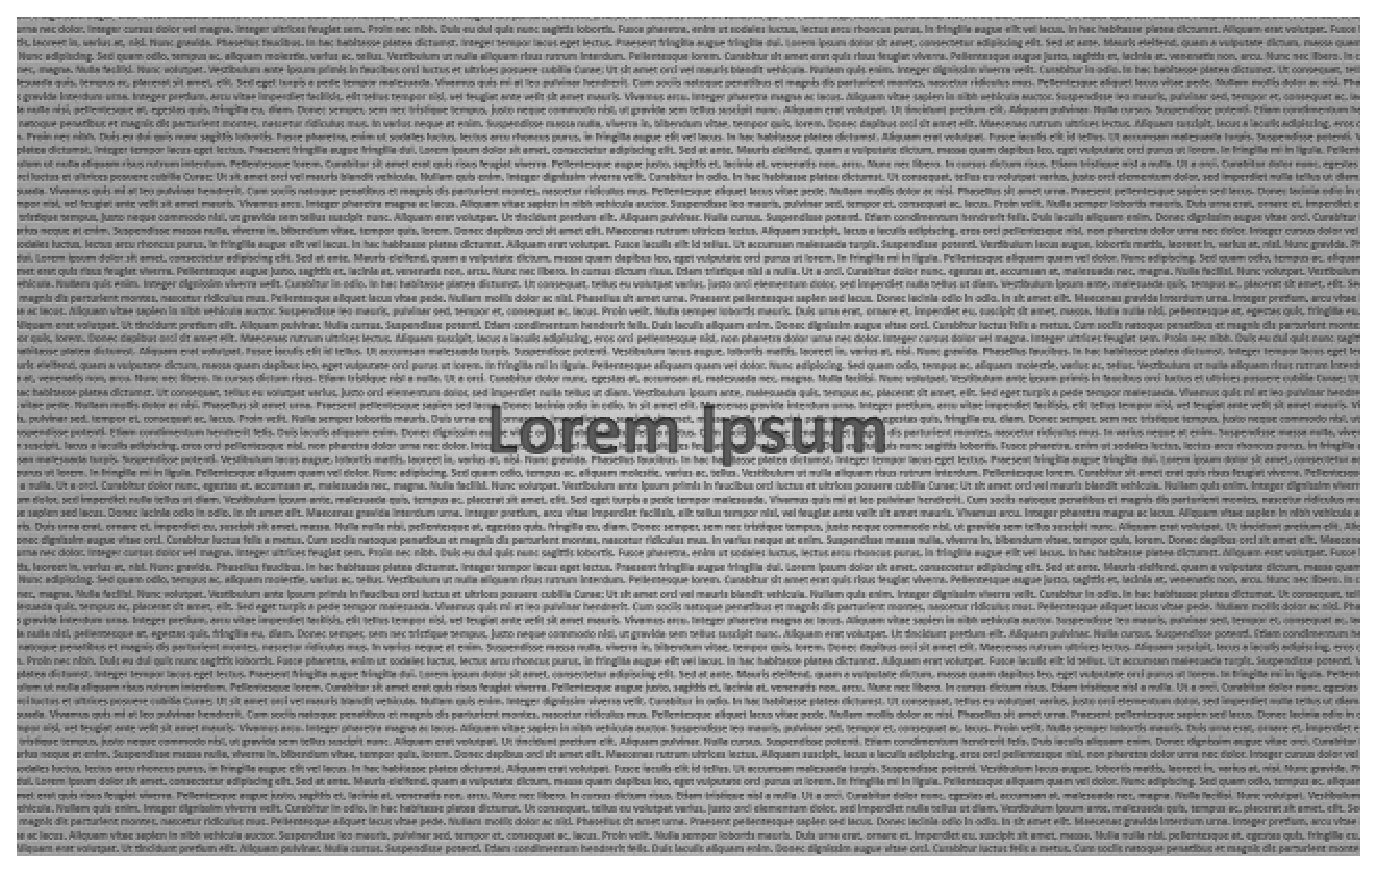
\includegraphics[width=0.6\textwidth]{Koopmans_Bernardi/01x02}
%\end{center}
%\caption{This is figure 2 in chapter 1.}
%\end{figure}


\bibliographystyle{plain}
\bibliography{Koopmans_Bernardi/References}


